\section{Stowage capacity case study}\label{sec:results}
\subsection{Stowage model}
In this section we present the stowage model that is the point of origin for our projected capacity model. In other words, this model describes the (in)equality system which we want to project. The model is adapted from the PhD thesis of Delgado \cite{AlbertosThesis}; other models for stowage planning using actual vessel profiles can be found in e.g. \cite{DariosThesis}, \cite{pacino11} and \cite{pacino12}. We will not go into details of the model in this report, but will only present the essentials; the reader is referred to \cite{AlbertosThesis}  
for further details. 
%
%%%%%%%%%%%%%%%%%%%%%%%%%%%%%%%%%%%%%
\subsubsection*{Description}
As shown in Figure~\ref{fig:vessel}, the cargo space of a container vessel is divided into
sections called \textit{bays} that each are divided into a grid by stacks and tiers (Figure~\ref{fig:bay_a}). Each stack and tier constitute a \emph{cell} that consists of two \emph{slots}. 

\begin{figure*}[tbh]
  \centering
  $\qquad$
	\subfloat[]{\label{fig:vessel} 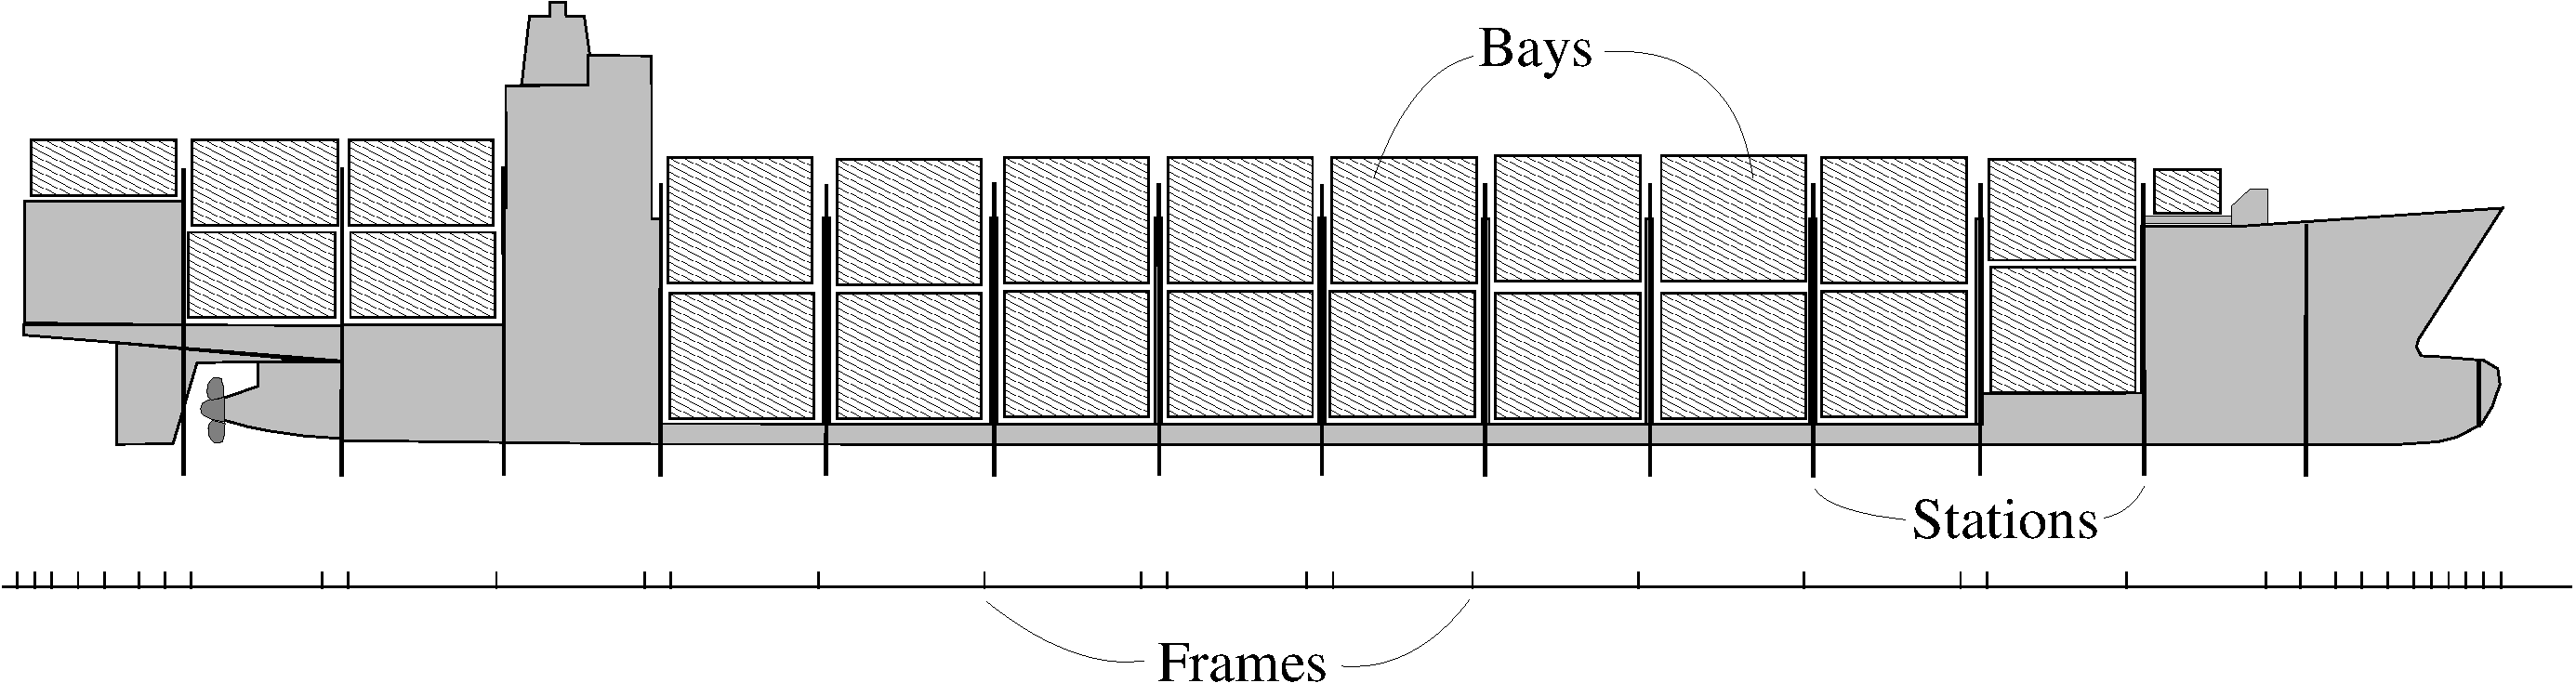
\includegraphics[scale=0.3]{figures/vesselBlocks.pdf}}\\
  \subfloat[]{\label{fig:bay_a} 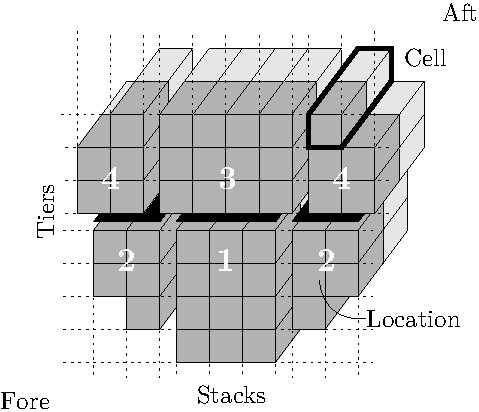
\includegraphics[scale=0.65]{figures/bay1.pdf}}~
	\qquad
  \subfloat[]{\label{fig:bay_b}  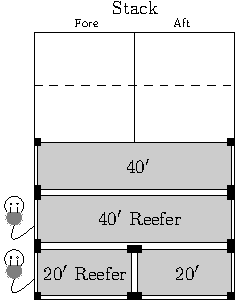
\includegraphics[scale=0.8]{figures/stack1.pdf}}~
  $\qquad$
\caption{(a) The arrangement of bays in a small container vessel. (b) A bay divided into cells given by stacks and tiers. The cells are grouped into four locations. (c) A side view of a stack of containers with power plugs for reefer containers at bottom slots. {Adapted from \cite{AlbertosThesis}.}}
\label{fig:bay}
\end{figure*}

The containers transported on a vessel usually have a standard size that fits the cells and slots; the containers are normally (ISO standard) $8'$ wide, $8'6''$ high and $20'$,
$40'$ or $45'$ long, though we do not consider the latter in this report. Accordingly, a cell can hold either two $20'$ containers (one in each slot) or one $40'$ container (Figure~\ref{fig:bay_b}). Further, some containers are refrigerated (\emph{reefers}), and must be stowed at a power plug. 
The corners of the containers are constructed such that containers can be stacked, though $20'$ containers cannot
be stacked on top of $40'$ containers due to the lack of corner supports in the middle of $40'$ containers (see Figure~\ref{fig:bay_b}). 

The capacity of a container vessel is measured in \emph{TEU} (Twenty-foot Equivalent Units), i.e. a standard $20'$ container as described above takes up one TEU, while a $40'$ container takes up two TEU. Each stack has a height and weight limit. Separate total weight limits for $20'$ and $40'$ containers exist, since only $20'$ containers rest on the middle support sockets of the stack, while the end sockets hold weight of both $20'$ and $40'$ containers (see Figure~\ref{fig:bay_b}). 

Though containers physically are placed in specific slots, the stowage models considered here are themselves abstractions called master plans that specify how many containers of each \emph{type} should be stowed in each subsection of each bay, referred to as a {\em location}. These locations emerge by dividing the bays {vertically} into sections on deck and below deck, respectively, and {horizontally} into a center section and symmetric side-sections, respectively; see Figure~\ref{fig:bay_a} which shows a bay divided into four location indicated by their number. The type of containers is here specified by the length, reefer-property and a weight class. The capacities for stacks translate to capacities for locations.

Besides the location-based capacity constraints, global hydrostatic constraints ensure the stability of the vessel. Stress forces arise as a result of gravitation acting downwards on the vessel and buoyancy acting upwards. The gravity forces are divided into three components: the light ship (i.e, the vessel mass without cargo and ballast water), cargo, and ballast water. Buoyancy forces are due to the vessel's displacement of water and hence depends on the varying (and irregular) shape of the hull, which is given at a set of reference points called \emph{stations} (see Figure~\ref{fig:vessel}). At these stations, the area submerged in water can be approximated by linear functions of the vessel's  longitudinal center of gravity (\emph{lcg}), and from this an approximation of the buoyancy force of the vessel between two consecutive stations can be calculated.~\footnote{A more accurate buoyancy model also takes the displacement of the vessel into account.}

There are three major stress forces: shear force, bending moment, and torsion moment. Limits on these stress forces are given for a set of points along the vessel called \emph{frames} (see Figure~\ref{fig:vessel}). In this work we only consider the limits on shear forces.

\subsubsection*{Sets, variables, constants}
To formally describe the stacking and stability constraints of the considered stowage models, we use the sets, variables and constants summarized in Table~\ref{table:sets}, Table~\ref{table:vars} and Table~\ref{table:constants}, respectively.
\begin{table}[p]
\centering
\begin{tabular}{p{5cm}p{7.5cm}}%p{2cm}}
\multicolumn{2}{l}{\textbf{Sets}}\\
\hline\noalign{\smallskip}
$L$ 
	& Set of locations.\\
$\Sec$
	&Set of frames.\\
$\Sec^{\trt{f}},\Sec^\trt{a}\subseteq \Sec$
	&Sets of frames \emph{fore} and \emph{aft} where shear force limits must hold.\\
$S, S' = \{s_1,\ldots, s_S\}$ 
	&Number of stations and (ordered) set of stations.\\
$T$
	&Set of types of containers.\\ 
$T^\trt{20}$, $T^\trt{40}$, $T^\trt{R}$, $T^\trt{20R}$, $T^\trt{40R}\subseteq T$ 
	&Set of types that are $20'$ long, $40'$ long, reefers, $20'$ reefers, and $40'$ reefers, respectively.\\ 
$\mi{BT}$ 
	& Set of ballast tanks.\\
\end{tabular}
\caption{Sets used in the considered stowage models.}
\label{table:sets}
\end{table}
%
\begin{table}[p]
\centering
\begin{tabular}{p{3.5cm}p{9cm}}
\multicolumn{2}{l}{\textbf{Decision variables}}\\
\hline
$x_{l,\tau}\in \mathbb{R}^+_0$
		&Number of containers of each type $\tau\in T$ to be stowed at each location $l\in L$.\\
$x_b\in \mathbb{R}^+_0$
		& The weight of each ballast tank $b\in \mi{BT}$.\\
\\
\multicolumn{2}{l}{\textbf{Auxilliary variables}}\\
\hline
$\weight_l\in \mathbb{R}^+_0$
		&The weight of all containers stowed at each location $l\in L$.\\
$x_\tau\in \mathbb{R}^+_0$
		&The total number of containers of each type $\tau\in T$.\\
$\shear_f\in \mathbb{R}$
		&{The shear force at each frame $f\in \Sec$}.\\
$lcg\in\mathbb{R}$
		&{The longitudinal center of gravity}.\\
$\bonjean_s \in\mathbb{R}$
		&{The buoyancy force at each section between station $s\in S'\setminus\{s_S\}$ and the next station.}\\
$\shear_f^{\trt{c},e}$, $\shear_f^{\trt{bt},e}$, $\shear_f^{\trt{bc},e}\in\mathbb{R}$
		&The contribution to the shear force for/aft (${e}\in\{\trt{f},\trt{a}\}$) each frame $f\in\Sec$ from containers (\trt{c})/ballast tanks (\trt{bt})/buoyancy (\trt{bc})
\end{tabular}
\caption{Variables used in the considered stowage models.}\label{table:vars}
\end{table}
Regarding the variables, we note that even though $x_{l,\tau}$ is a number of containers and hence a natural number, we model it as a reel number to ensure that the resulting model is an LP. Due to the large number of containers that can be stowed in each location, this approximation is sufficiently accurate in practice. 
%
\begin{table}[p]
\centering
\begin{tabular}{p{4.5cm}p{8cm}}%p{2cm}}
\multicolumn{2}{l}{\textbf{Constants}}\\
\hline\noalign{\smallskip}
$\Ca_l^\trt{20}$, $\Ca_l^\trt{40}$, $\Ca_l^\trt{TEU}$, $\Ca_l^\trt{RS}$, $\Ca_l^\trt{RC}$, 
$\Ca_l^\trt{W20}$, $\Ca_l^\trt{W40}$
		& The capacity for each location $l\in L$, w.r.t. $20'$ containers, $40'$ container, TEU, reefer slots, reefer cells, weight of $20'$ containers, and weight of $40'$ containers, respectively.\\
%\hline
$\Weight_\tau$
		&The weight of a type of container $\tau\in T$.\\
%\hline
$\Bonj^\trt{lcg}_s$, $\Bonj^\trt{C}_s$
		&{Coefficients for the linearization of the submerged area at each station $s\in S'$.}\\
%\hline
$D_s$ &
		The distance between $s\in S'\setminus\{s_S\}$ and the next station.\\
%\hline
$W^\trt{f}_f$, $W^\trt{a}_f$
		&{The constant weight of the vessel fore/aft each frame $f\in\Sec$ (light ship)}\\
%\hline
$\Prop^{e}_{f,l}$, $\Prop^{e}_{f,b}$, $\Prop^{e}_{f,s}\in [0,1]$
		& The fraction of each location $l\in L$/ballast tank $b\in \mi{BT}$/section between $s\in S'\setminus\{s_S\}$ and the next station that lies fore/aft (${e}\in\{\trt{f},\trt{a}\}$) each frame $f\in\Sec$.\\
%\hline
$\mi{UB}(\mi{lcg})$, $\mi{lb}(\mi{lcg})$,\newline $\mi{UB}(\mi{sf}_f)$, $\mi{lb}(\mi{sf}_f)$,\newline 
 $\mi{UB}(x_b)$, $\mi{UB}(\trt{WBT})$,\newline $\mi{lb}(\trt{WBT})$
		&The upper and lower bounds for the lcg, shear force at each frame $f\in \Sec$, the weight for each ballast tank $b\in BT$ (upper bound only), plus 
		the weight of ballast tanks in total, respectively.\\
\end{tabular}
\caption{Constants used in the considered stowage models}\label{table:constants}
\end{table}
%
\subsubsection*{Constraints}
\paragraph{Location-based capacity constraints}
Firstly, we have constraints that ensure that for each location of the vessel, the stowed containers are within the allowed capacities w.r.t. the number of $20'$ containers, $40'$ containers, TEUs, and the weight of the $20'$ and $40'$ containers, respectively. These constraint are modeled in the inequalities \eqref{20Cap}-\eqref{weight40Cap} below.
{Likewise, we have a constraint, \eqref{combinedWeightCap}, that ensures that the weight of a location is within limits, taken the different distribution of the weight of $40'$ containers, respectively $20'$ containers, within a slot into consideration; the weight of a $40'$ container is distributed on the four outer corner places of a slot while the weight of $20'$ containers also rest on the inner corners of the slot.}
Lastly, \eqref{reeferSlotCap} and \eqref{reeferCellCap} ensure that each reefer container can be refrigerated, and that {the total number of cells taken up by the reefer containers are within capacity}, respectively. 
\begin{align}
{\forall l \in L:}&\quad
	%\tag{$20'$ capacity}
	\label{20Cap}
	{\sum_{\tau \in T^\trt{20}} x_{l,\tau} \leq \Ca_l^\trt{20}}\\
%
%\tag{$40'$ capacity}
\label{40Cap}    	
	{\forall l \in L:}&\quad
	{\sum_{\tau \in T^\trt{40}} 2\cdot x_{l,\tau} \leq \Ca_l^\trt{40}}\\
%
%\tag{TEU capacity}
\label{teuCap}
	\forall l \in L:&\quad
	\sum_{\tau \in T^\trt{20}} x_{l,\tau} + 2\cdot\sum_{\tau \in T^\trt{40}} x_{l,\tau} \leq \Ca_l^\trt{TEU}\\
%
%\tag{Volume capacity}
%\label{volCap}
%{\forall l \in L:&\quad\sum_{\tau \in T} \Vol_\tau\cdot x_{l,\tau} \leq \Ca_l^\trt{vol}}\\
%
%Weight vars and weight capacity
%\tag{$20'$ weight capacity}
\label{weight20Cap}
	\forall l \in L:&\quad\sum_{\tau \in T^\trt{20}} \Weight_\tau\cdot x_{l,\tau} \leq \Ca_l^\trt{W20}\\
%
%\tag{$40'$ weight capacity}
\label{weight40Cap}
	\forall l \in L:&\quad\sum_{\tau \in T^\trt{40}} \Weight_\tau\cdot x_{l,\tau} \leq \Ca_l^\trt{W40}\\
%
%\tag{Combined weight capacity}
\label{combinedWeightCap}
	\forall l \in L:&\quad 0.5\cdot \sum_{\tau \in T^\trt{20}} \Weight_\tau\cdot x_{l,\tau} + \sum_{\tau \in T^\trt{40}		} \Weight_\tau\cdot x_{l,\tau} \leq \Ca_l^\trt{W40}\\
%
%\tag{Reefer slot capacity}
\label{reeferSlotCap}
	\forall l \in L:&\quad\sum_{\tau \in T^\trt{R}} x_{l,\tau} \leq \Ca_l^\trt{RS}\\
%
%\tag{Reefer cell capacity}
\label{reeferCellCap}
	{\forall l \in L:}&\quad
	{\sum_{\tau \in T^\trt{20R}} 0.5\cdot x_{l,\tau} + \sum_{\tau \in T^\trt{40R}} x_{l,\tau} \leq \Ca_l^\trt{RC}}
%   	
%//Type capacity constraint
%\label{typesConstraints}
%\red{\forall l \in L, \tau \in T:}&\quad
%\red{\sum_{\tau' \in TypesConstraint_\tau} x_{l,\tau'} \leq LocationsTypesCap_{l,\tau}}\\
\end{align}	 
%
\paragraph{Defined variables and bounds}
The constraint in \eqref{typeDef} defines the variables, $x_\tau$, that specifies how many containers of a specific type $\tau$ is stowed on the vessel. These are the variables that we want the projected (in)equality system to be expressed in.
\begin{equation}
\label{typeDef}%\tag{Type definition}
	\forall{\tau \in T}: x_\tau = \sum_{l\in L} x_{l,\tau}
\end{equation}
\eqref{totalWeightDef} below defines the total weight of the containers stowed in each location, since this number is used in further calculations of the hydrostatic constraints (see further below). 
\begin{equation}
%\tag{Total weight definition}
\label{totalWeightDef}
	\forall l \in L:\quad \weight_l = \sum_{\tau \in T} \Weight_\tau\cdot x_{l,\tau}\\
\end{equation}
We also ensure that the number of containers placed at each location of each type as well as the amount of ballast in the ballast tanks is positive. 
For the ballast tanks, we also require that each tank's content is within limits, as well as the total content. These constraints are given in \eqref{btLim} and \eqref{BTLim} below.
\begin{align}
\label{xPos}
	\forall l\in L, \tau\in T:&\quad 0\leq x_{l,\tau}.\\
%\tag{Limits for each tank}
\label{btLim}
	\forall b \in BT:	&\quad 0 \leq x_b \leq \mi{UB}(x_b)\\ 
%
%\tag{Limits for total weight of tanks}
\label{BTLim}
	\mi{lb}(\trt{WBT}) &\leq \sum_{b \in BT} x_b	\leq \mi{UB}(\trt{WBT})
\end{align}
%
\paragraph{Hydrostatic constraints}
%For vessel stability, the model in \cite{AlbertosThesis} uses variable displacement, and for this it uses discrete displacement intervals. To avoid integer variables we consider here a constant displacement interval, and we assume that the stowed containers lie within $75$ to $85$ percent of the vessel's maximal allowable displacement. 
At each station, the submerged area of the cross-section has been linearized as a function of the lcg, and the buoyancy force for each section between consecutive stations are calculated as the average of the two areas times the distance between the two stations \eqref{bonjeanVarDef}. 
Instead of calculating the vessel's lcg, we only require it to be within a given interval \eqref{lcgLim}.

The shear forces must be within limits for a set of fore ($\Sec^{\trt{f}}$) and aft ($\Sec^\trt{a}$) frames. The shear force for a fore frame is the sum of resulting forces acting from the frame towards the stern, while the shear force for an aft frame is the sum of resulting forces acting from the frame towards the bow of the vessel, see \eqref{eq:shear}. For each of the frames, we then require these shear forces to be within limits \eqref{shearLimits}.

\begin{gather}
\forall s_i \in S'\setminus\{s_S\}:\;
\bonjean_{s_i} = \frac{1}{2}\cdot D_{s_i}\cdot(\Bonj^\trt{C}_{s_i} + \mi{lcg}\cdot \Bonj^\trt{lcg}_{s_i}	+ \Bonj^\trt{C}_{s_{i+1}} + \mi{lcg}\cdot \Bonj^\trt{lcg}_{s_{i+1}})
\label{bonjeanVarDef}\\
%
\mi{lb}(\mi{lcg}) \leq \mi{lcg} \leq \mi{UB}(\mi{lcg})
\label{lcgLim}\\
%
\forall {e}\in\{\trt{f},\trt{a}\}, f \in \Sec^{e}:\;
\shear_f = W^{e}_f+ \sum_{l\in L} \weight_l\cdot \Prop_{f,l}^{e} + \sum_{b \in BT} x_b\cdot \Prop^{e}_{f,b} 	+ \smashoperator{\sum_{s_i \in S'\setminus\{s_S\}}}\bonjean_{s_i}\cdot \Prop^{e}_{f,s_i}
\label{eq:shear}\\
%
\forall f \in \Sec:\;	\mi{lb}(\shear_f)\leq	\shear_f \leq \mi{UB}(\shear_f)
\label{shearLimits}
\end{gather}
%
\subsection{Experimental results}\label{sec:testResults}
To do a nested decomposition (see section \ref{sec:nested}), we will, though, divide the constraints in \eqref{eq:shear} in a part coming from the containers, ballast tanks and bouyancy, respectively, using auxiliary variables. Thus \eqref{eq:shear} is replaced with \eqref{shearLocDef}-\eqref{shearDef} below.
\begin{align}
\label{shearLocDef} 
\forall {e}\in\{\trt{f},\trt{a}\}, f \in \Sec^{e}:&\;
	\shear^{\trt{c},e}_f = \sum_{l \in L} \weight_l\cdot \Prop^{e}_{f,l}\\
%
\forall {e}\in\{\trt{f},\trt{a}\}, f \in \Sec^{e}:&\;
	\label{shearTanksDef}
	\shear^{\trt{bt},e}_f = \sum_{b \in \mi{BT}} x_b\cdot \Prop^{e}_{f,b} \\		
%
\forall {e}\in\{\trt{f},\trt{a}\}, f \in \Sec^{e}:&\;
	\label{shearBonjDef}
	\shear^{\trt{bc},e}_f = \sum_{s_i \in S'\setminus\{s_S\}} \bonjean_{s_i}\cdot \Prop^{e}_{f,s_i} \\
%
\forall {e}\in\{\trt{f},\trt{a}\}, f \in \Sec^\trt{e}:&\;
	\label{shearDef}
 	\shear_f = W^{e}_f +	\shear^{\trt{c},e}_f+ \shear^{\trt{bt},e}_f + \shear^{\trt{bc},e}_f
\end{align}

We have tested our methods on three different models, each including a different number of the constraints presented in the previous section and above. In all cases, we wanted a model capturing all the dependencies between the  variables $x_\tau$, and only those. Hence we project the variables $\VAR(S)\setminus \set{x_\tau}{\tau\in T}$ where $S$ is the system consisting of the (in)equalities corresponding to the constraints of the model.

We have used data from our industrial partner, Maersk, from a vessel with a capacity of $15.500$ TEU, $91$ locations, $27$ ballast tanks and $33$ stations. There are $25$ frame points, however, we have only used one fore and one aft (in the two models considering hydrostatics). In all models, we considered 12 types, $T = \{20', 40'\}\times \{6t, 21t, 27t\}\times\{\trt{R}, \trt{NR}\}$, that are defined according to the length, the weight class and the reefer property of the containers.

In the two tables below we show which (in)equalities are present in the 3 (in)equality systems $S_1$, $S_2$ and $S_3$ that have been tested, and we state the size of each model given in number of (in)equalities, number of variables and the two numbers multiplied. Similarly we present the size of the projected (in)equality systems together with the approximate time taken to obtain those projections. 

The (in)equality system $S_1$ includes $3$ capacity constraints per location and shear force calculations at $2$ frame points; $S_2$ includes all capacity constraints for each location but no calculations of shear forces. $S_3$ includes 6 capacity constraints per location and shear force calculations at the two frames.

\begin{table}[H]
\centering
{\renewcommand{\arraystretch}{1.2}
\begin{tabular}[t]{l|p{9cm}}
(In)eq. system&Constraints included\\
\hline
$S_1$& \eqref{teuCap}, \eqref{combinedWeightCap}, \eqref{reeferCellCap}, \eqref{typeDef}, \eqref{totalWeightDef}, \eqref{xPos}, \eqref{btLim}, \eqref{BTLim}, \eqref{bonjeanVarDef},  \eqref{lcgLim}, \eqref{shearLimits}, {\eqref{shearLocDef}}, \eqref{shearTanksDef}, \eqref{shearBonjDef}, \eqref{shearDef}\\
\hline
$S_2$&\eqref{20Cap}, \eqref{40Cap}, \eqref{teuCap}, \eqref{weight20Cap}, \eqref{weight40Cap}, \eqref{combinedWeightCap}, \eqref{reeferSlotCap}, \eqref{reeferCellCap}, \eqref{typeDef}, \eqref{totalWeightDef}, \eqref{xPos}\\
\hline
$S_3$& \eqref{20Cap}, \eqref{40Cap}, \eqref{teuCap}, \eqref{combinedWeightCap}, \eqref{reeferSlotCap}, \eqref{reeferCellCap},  \eqref{typeDef}, \eqref{totalWeightDef}, \eqref{xPos}, \eqref{btLim}, \eqref{BTLim}, \eqref{bonjeanVarDef}, \eqref{lcgLim}, \eqref{shearLimits}, {\eqref{shearLocDef}}, \eqref{shearTanksDef}, \eqref{shearBonjDef},  \eqref{shearDef}\\
\end{tabular}
}
\caption{Constraints included in test systems.}\label{fig:constraints}
\end{table}

The tests have been done on a laptop with an Intel$^\text{\textregistered}$ Core\texttrademark\; i7-4600U-processor with a frequency of 2.10-3.3 GHz, 8GB RAM, and with $2$ cores and $4$ threads. The computer has also been used to perform other tasks while doing the projection, and $3$ threads were used to run the parallel redundancy checks. The time used to make the projection is therefore not accurate, but still gives an indication of the running time (especially when these are compared across the test results). 

\begin{table}[H]
\centering
\noindent\begin{tabular}{|l|r|r|r|r|r|r|r|}
\hline
(In)equality&App. time&\multicolumn{3}{c|}{Size of system}&\multicolumn{3}{c|}{Size of projected system}\\
system&&{\#(in)eqs}&{\#vars}&${\#\text{ineqs}\cdot\#\text{vars}}$&{\#(in)eqs}&{\#vars}&${\#\text{ineqs}\cdot\#\text{vars}}$\\
%\scriptsize{\#vars}&$\substack{\#\text{ineqs}\quad\\\cdot\#\text{vars}}$\\
\hline
$S_1$&6 m&537&1092&586,404&26&12&312\\
$S_2$&18.5 h&922&1209&1,114,698&42&12&504\\
$S_3$&97 h&811&1171&949,681&106&12&1272\\
\hline
\end{tabular}
\caption{Sizes of original and projected systems.}\label{tab:results}
\end{table}

In all three test cases, the system consisting of the (in)equalities using $x_{l,\tau}$ and $\weight_l$ were set aside; this is the system corresponding to the constraints \eqref{20Cap}-\eqref{xPos} (for $S_2$) plus \eqref{shearLocDef} (for $S_1$ and $S_3$). Then these systems were decomposed according to the locations, and the variables $x_{l,\tau}$ and $\weight_l$ were eliminated, leaving a system over $x_\tau$ (for $S_1$), or $x_\tau$ and $\shear^{\trt{c},e}_f$ (for $S_1$ and $S_3$). The decomposition was done such that $X_i = \set{x_{l,\tau}}{\tau \in T, l\in P^0_i}\cup\set{\weight_l}{l\in P^0_i}$ for each $1\leq i \leq 45$, where  
\begin{align*}
(P^0_1,P^0_2,\ldots, P^0_{45}) =
&\big(\{0,1,2\}, \{3,4\}, \{5,6\}, \{7,8\}, \{9,10\}, \{11,12\}, \{13,14\}, \{15,16\}, \{17,18\}, \\
&\{19,20\}, \{21,22\},\{23,24\}, \{25,26\}, \{27,28\}, \{29,30\}, \{31,32\}, \{33,34\}, \\
&\{35,36\}, \{37,38\}, \{39,40\}, \{41,42\}, \{43,44\}, \{45,46\}, \{47,48\}, \{49,50\}, \\
&\{51,52\}, \{53,54\}, \{55,56\}, \{57,58\}, \{59,60\}, \{61,62\}, \{63,64\}, \{65,66\}, \\
&\{67,68\}, \{69,70\}, \{71,72\}, \{73,74\}, \{75,76\}, \{77,78\}, \{79,80\}, \{81,82\}, \\
&\{83,84\}, \{85,86\}, \{87,88\}, \{89,90\}, \{91\}\big).
\end{align*}

For $S_1$ and $S_3$, the list of partitions $\mathfrak{P}$ was $\mathfrak{P} = (\mathbb{P}^1, \mathbb{P}^2, \mathbb{P}^3, \mathbb{P}^4, \mathbb{P}^5)$, where 
\begin{align*}
\mathbb{P}^1 &= \big( \{0,1\}, \{2,3\}, \{4,5\}, \{6,7\}, \{8,9\}, \{10,11\}, \{12,13\}, \{14,15\}, \{16,17\},\\
						 & \quad \{18,19\}, \{20,21\}, \{22,23\}, \{24,25\}, \{26,27\}, \{28,29\}, \{30,31\}, \{32,33\},\\
						 & \quad \{34,35\}, \{36,37\}, \{38,39\}, \{40,41\}, \{42,43\}, \{44,45\} \big),\\
\mathbb{P}^2 &= \big( \{0,1\}, \{2,3\}, \{4,5\}, \{6,7\}, \{8,9\}, \{10,11\}, \{12,13\}, \{14,15\}, \{16,17\},\\
						 & \quad \{18,19\}, \{20,21\}, \{22\} \big),\\
\mathbb{P}^3 &= \big( \{0,1\}, \{2,3\}, \{4,5\}, \{6,7\}, \{8,9\}, \{10,11\} \big),\\
\mathbb{P}^4 &= \big( \{0,1\}, \{2,3\}, \{4,5\} \big),\\
\mathbb{P}^5 &= \big(\{0\}, \{1,2\} \big).
\end{align*}

For $S_2$, the partitions where $\mathfrak{P}' = (\mathbb{P}'^1, \mathbb{P}'^2, \mathbb{P}'^3, \mathbb{P}'^4, \mathbb{P}'^5)$, where 
\begin{align*}
\mathbb{P}'^1 &= \mathbb{P}'^1,\\  
\mathbb{P}'^2 &= \big\{ \{0,1\}, \{2,3\}, \{4,5\}, \{6,16\}, \{8,9\}, \{10,18\}, \{12,13\}, \{14,15\}, \{7,17\},
						   \{11,19\},\\
							& \quad \{20,21\}, \{22\} \big\},\\
\mathbb{P}'^3 &= \big\{ \{0,2\}, \{1,3\}, \{4,6\}, \{5,7\}, \{8,10\}, \{9,11\} \big\},\\
\mathbb{P}'^4 &= \big\{ \{0,1\}, \{2,4\}, \{3,5\} \big\},\\
\mathbb{P}'^5 & = \mathbb{P}^5.
\end{align*}

The reason for having $\mathfrak{P}'$ like this (and not just ``numerical'') was to ``pair'' partitions according to the size of the produced (sub)projections such that some of the smaller projections were paired with some of the larger projection. The reason that some of the (sub)projections were smaller is partly that some of the locations have no reefer capacity, so $x_{l,\tau}$ for such a location and a $\tau$ that is a reefer type is quickly set to $0$, which makes the projection smaller.

For $S_2$, making the above projection resulted in the required system expressed only in the $x_\tau$-variables.

For both $S_1$ and $S_3$ we projected yet two more subsystems; the subsystem consisting of the (in)equalities relating to buoyancy (\eqref{bonjeanVarDef}, \eqref{lcgLim}  and \eqref{shearBonjDef}) were projected w.r.t. $lcg$ and $\bonjean_s$ (leaving only the $\shear^{\trt{bc,f}}_f$ and $\shear^{\trt{bc,a}}_f$ variables), while the subsystem relating to ballast tanks (\eqref{btLim}, \eqref{BTLim} and \eqref{shearTanksDef}) were projected w.r.t. $x_b$ (leaving the $\shear^\trt{bt,f}_f$ and $\shear^\trt{bt,a}_f$ variables). 
For both $S_1$ and $S_3$, the three projected subsystems were then joined together with the (in)equalities \eqref{shearLimits} and \eqref{shearDef}, relating to the shear force. In this final system, we then eliminated the $\shear^{\trt{c},e}_f$, $\shear^{\trt{bt},e}_f$, $\shear^{\trt{bc},e}_f$, and the $\shear_f$-variables, which resulted in a system over the $x_\tau$-variables as required. 
%\marginpar{Actually, we had the \eqref{shearLocDef} included in the ``container''-part, but I am not sure if this makes a difference}

\begin{figure}[p]
	\centering
		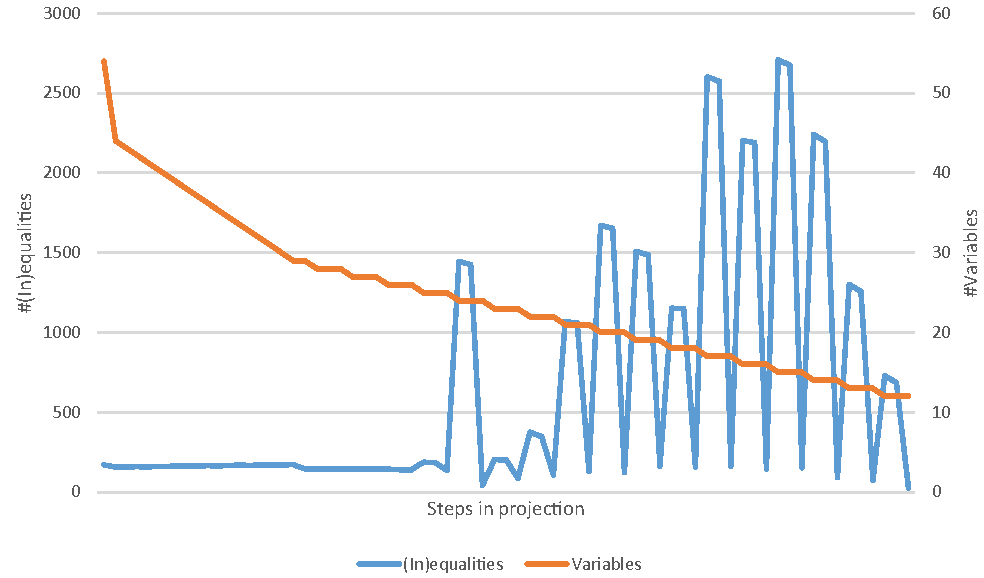
\includegraphics[scale=0.6]{figures/FinalProjection-29-2Shear.pdf}
	\caption{Projection of the final system stemming from $S_1$. }
	\label{fig:FinalProjectionS1}
\end{figure}

\begin{figure}[p]
	\centering
		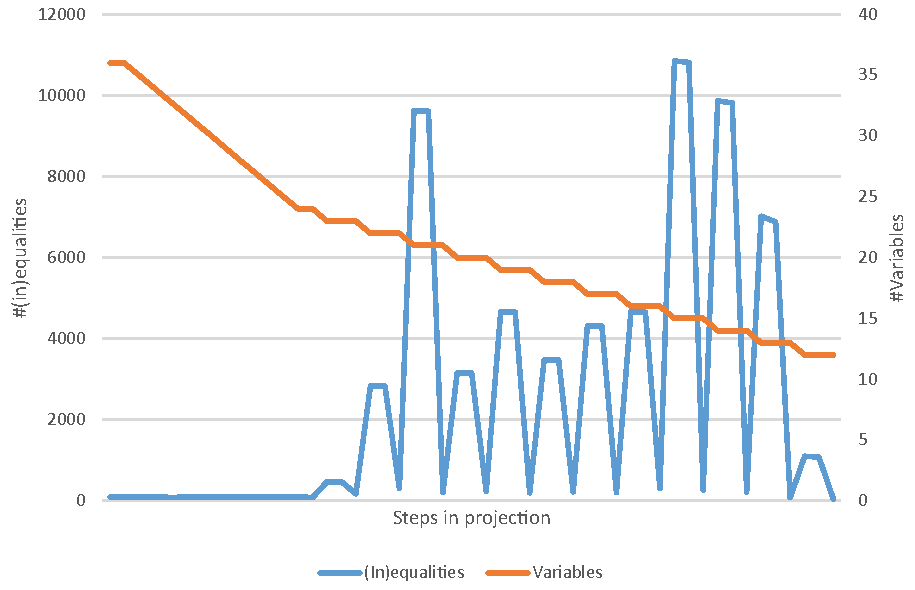
\includegraphics[scale=0.6]{figures/FinalProjection-24.pdf}
	\caption{Projection of the final system stemming from $S_2$. }
	\label{fig:FinalProjectionS2}
\end{figure}

\begin{figure}[p]
	\centering
		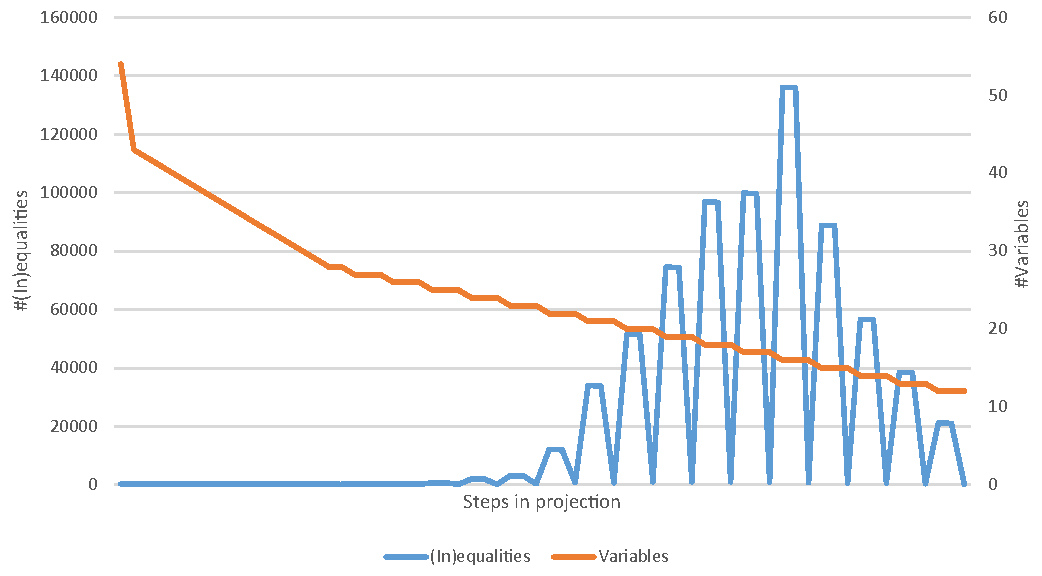
\includegraphics[scale=0.6]{figures/FinalProjection-30.pdf}
	\caption{Projection of the final system stemming from $S_3$. }
	\label{fig:FinalProjectionS3}
\end{figure}

To give the reader an idea of the how the number of (in)equalities and variables, respectively progress, Figure~\ref{fig:FinalProjectionS1}, Figure~\ref{fig:FinalProjectionS2} and Figure~\ref{fig:FinalProjectionS3} show the evolution of these numbers when projecting the mentioned final system stemming from $S_3$, which is the system producing the largest intermediary systems. Each ``step'' in these graphs corresponds to either the preprocessing or ''clean-up'' (as a whole), Gauss-elimination of one variable, FM-elimination of one variable, or a complete redundancy removal of the system. The first part where the number of (in)equalities is reasonable stable (when seen in this scale) corresponds to the preprocessing and Gauss-elimination part. 
This is followed by repeated steps of FM-elimination (the ``peaks'' in the number of (in)equalities), clean-up (the ``flat'' part after the peaks) and redundancy removal (the ``valleys'').

We note that $S_3$ is the most time-consuming system to project of the three, and the final system as shown in Figure~\ref{fig:FinalProjectionS3} is by far the system (of all the subsystems that were projected) that produced the biggest intermediary systems.  

\subsection{Implementation notes}
In the following we will give a few remarks regarding the specifics of the implementation.

The program was implemented in Java, and we use rationals for the coefficients and right-hand-sides.
In the implementation, we have used a list, not a set, for representing the (in)equalities in a system. Thus, at a given point, the (in)equality system $S$ might contain two (in)equalities $c$ and $c'$ for which $\vea(c)=\vea(c')$ and $\rhs(c)=\rhs(c')$. However, either $c$ or $c'$ will be removed in the preprocessing/clean up step (when removing linearly dependent (in)equalities), and this does not influence the correctness of the algorithm(s).
We also normalize the (in)equalities in the inequality system such that the smallest absolute value of the coefficients is $1$. This also makes it easier to detect linear dependencies. 

$\epsilon$ in Section~\ref{sec:uncertainty} is set to $0.01$, $\epsilon' = 0.000001$, and $\mathcal{K} = 10^{14}$. The optimization software CPLEX from IBM was used as lp-solver. 
\\
\\
{We note that because we use the almost redundant criteria when doing (sequential) redundancy, the system $S'$ returned by \Call{RemoveRedundancy}{} in line~\ref{ln:projx} of Algorithm~\ref{alg:project} is no longer completely identical to $\proj_x(S)$; $S'$ will most likely be an overapproximation of the projection. However, as previously mentioned, the parameters of a problem -- and this indeed holds for the particular problem we have considered -- are not necessarily very accurate, and small discrepancies between the returned projection and the actual projection is acceptable. It still remains to be shown that the overapproximation is not ``too big'' according to a given criterion.}
\\
\\
Finally, we want to point out here, that the implemented program is non-deterministic due to a number of factors. 

Firstly, the almost redundant-criteria for removing inequalities in the sequential redundancy removal means that the order in which the inequalities are checked, matters. 
For two runs (on the same input system) to result in the exact  same projection, the variables must be projected in the same order, and at each variable elimination, the produced inequalities must be added in the same order (or checked for redundancy in the same order), and the redundancy check using CPLEX must result in the same yes/no answer (and $\kappa$-value). 
 
Making use of parallel redundancy check means that when an inequality from a system is checked for redundancy in two different runs, another inequality might have been deemed redundant by another checker and hence have been removed in one run, while it is not in the other run (because the checker finished later). This can influence how long the check of the current inequality takes and influence the $\kappa$-value, so this effect can propagate. In the end, this might cause the set of removed (in)equalities to vary in the two runs altogether (because some inequalities in reality are redundant but cannot be determined to be so). 

Likewise, we make use of an in-build mechanism in Java for parallelism, namely streams. These are used for example when using the heuristic for finding out which variable should be removed. Again, this can of course be avoided.

In conclusion, with careful ordering of variables e.t.c., settings of parameters for CPLEX and avoidance of parallelism, non-determinism could possibly be avoided, but will most likely also be less efficient.  
